\chapter{Hybrid dynamical systems}
	\de{Hybrid dynamical systems} are the ones that are allowed both in continuous and discrete-time, thus it's general state-space representation is in the form
	\begin{equation} \tag{H}
	\left\{\begin{aligned}
		\dx &  = \vet f(\x) \qquad &&\x \in \fset \qquad &&  \textrm{: continuous evolution} \\
		\xp & = \vet g(\x) \qquad &&\x \in \jset && \textrm{: discrete evolution}
	\end{aligned} \right.
	\end{equation}
	In this representation $\vet f$ is the \de{flow map} describing the evolution of the states in a continuous-time environment while $\x$ are in the \de{flow set} $\fset$; $\jset$ is instead the \de{jump set} and describe the \textit{region} of the states where the system is allowed to \textit{jump} with a discrete-time behaviour according to the \de{jump map} $\vet g$. Observe that in general $\fset \cup \jset \neq \mathds R^n$ and $\fset \cap \jset \neq \emptyset$.
	
	The simplest, yet effective, example is the one of a bouncing ball: given a point mass $m=1kg$ with states $(p,v)$ representing respectively the position and the velocity in the vertical direction (\textit{pointing upward} with respect to ground that's at $p=0$), then every-time the mass is above ground ($p>0$) it's allowed to flow according to the Newton equation. Calling so $\gamma =9.81N/kg$ the force/mass applied to the point mass, then the flow can be described as
	\[ \dx = \vector{\dot p \\ \dot v} = \vector{v \\ -\gamma} = \vet f(\x) \hspace{1.5cm} \x \in \fset = \big\{ \x = (p,v) \in \mathds R^2 \ : \ p \geq  0 \big\} \]
	When the ball finally reaches ground ($p=0$), when it's \textit{going downward} ($v<0$) then the bounce suddenly changes the direction of the speed (becoming positive); considering in general that in the shock some energy is lost, calling $\lambda \in [0,1]$ the so called \textit{restitution factor}, we can model the jumps of  the systems as
	\[ \xp = \vector{p^+ \\ v^+} = \vector{p \\ - \lambda v} = \vet g(\x) \hspace{1.5cm} \x \in \jset = \big\{ \x = (p,v) \in \mathds R^2 \ : \ p = 0 \textrm{ and } v \leq 0 \} \]
	
	While modelling hybrid systems, the definition of flow and jump set is of primary relevance; recalling this example, intuitively one other flow set could have been $\fset = \{ (p,v) \ : \ p > 0 \}$, however this comes the first \textit{requirement} that we won't prove (but is actually important while finding solutions of hybrid system): both \textbf{flow} and \textbf{jump} domains must be \de{close set}, so such that \textit{their boundaries are included}. Direct consequence of this choice is that $\fset$ and $\jset$ might \textit{overlap}, leading to a \textbf{non-unique solution} given the same initial condition.
	
\section{Solutions}
	\paragraph{Hybrid time domain} Given the mathematical description of an hybrid system, the associated solution must be parametrized in both continuous and discrete-time domain: for this reason we define the \de{hybrid time domain} $\hsol$ the subset of $\mathds R_{\geq 0} \times \mathds Z_{\geq 0}$ defined as
	\begin{equation} \label{eq:hyb:timedomain}
		\hsol = \bigcup_{j=0}^J I_j\times \{j\} \qquad \textrm{where } I_j = \big[t_j, t_{j+1} \big]
	\end{equation}
	where $j$ are the discrete-time jumps and $I_j = \big[t_j, t_{j+1}\big]$ are flow intervals between them. Possibly what we want in the solutions is $J\rightarrow \infty$ and that the last interval $I_j$ is \textit{open on the right}. Intuitively while regarding hybrid system we say that \textit{the time $t+j$ is always moving forward}. From this definition we call $t_0,t_1,\dots, t_j$ as the \textbf{jump times} and must satisfy
	\[ 0 = t_0 \leq t_1 \leq t_2 \leq \dots \leq t_J \] 
	
	\paragraph{Solution of a hybrid system} A \de{solution} of an hybrid system (H) is a \textbf{function} $\vet \phi(t, j)$ such that:
	\begin{enumerate}
		\item the domain of $\vet \phi(t,j)$ is an hybrid time domain as in (\ref{eq:hyb:timedomain});
		\item for each intervals $(t_1,j),(t_2,j) \in \textrm{dom}\{\vet \phi\}$ with $t_2> t_1$, then we must have
		\[ \tag{F} \frac{d}{dt} \vet \phi(t,j) = \vet f \big(\vet \phi(t,j)\big) \]
		and $\vet \phi(t,j) \in \fset$ is in the flow set for almost all $t\in [t_1,t_2]$ (excluding in particular the jump times);
		\item for each $(t,j), (t, j+1)\in \textrm{dom}\{\vet \phi\}$ then it must hold
		\[ \tag{J} \vet \phi(t, j+1) = \vet g\big(\vet \phi(t,j)\big) \]
		and $\vet \phi(t,j) \in \jset$ lies in the jump set.
	\end{enumerate}
	In general we regard (F) as the \de{flow condition} and (J) as the \de{jump}.
	
	Considering now an example of hybrid system characterized by the state-space representation
	\[ \tag{$\dagger$}\begin{cases}
		\dx = \vet f(\x) = \vector{1 \\ 1} \qquad & \x \in \fset = \overline{\mathds R^2\setminus \jset} \\
		\xp = \vet g(\x) = \vector{3/4 \\ 1/4} x_1 \qquad & \x \in \jset = \big\{ \x=(x_1,x_2) \in \mathds R^2 \ : \ 0 \leq 5x_2 \leq 2-x-1 \big\}
	\end{cases} \]
	some of its solution have been represented in figure \ref{fig:hyb:example}.
	\begin{figure}[bt]
		\centering 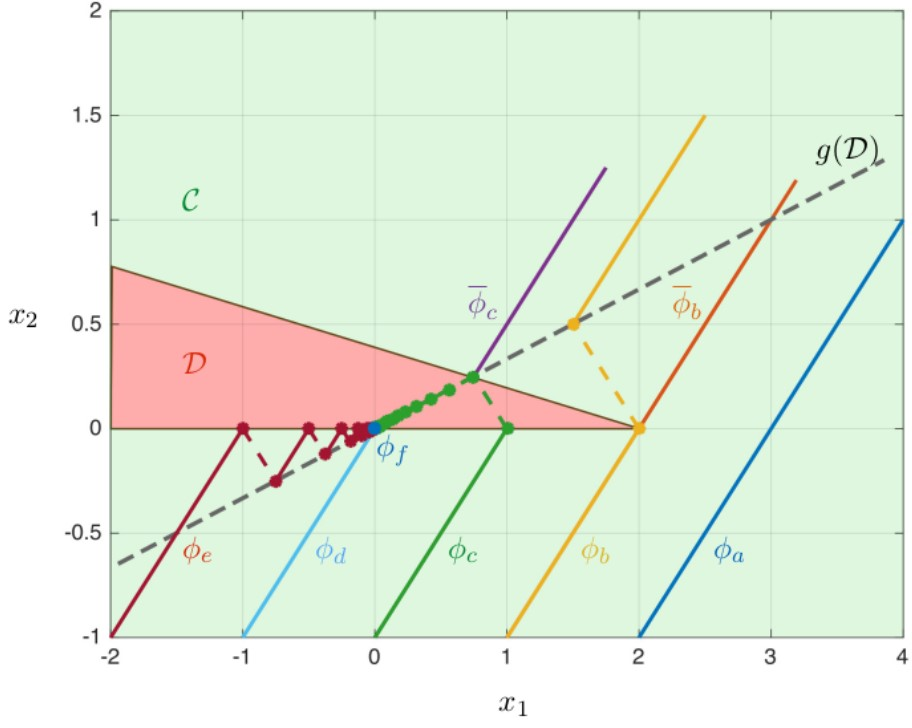
\includegraphics[width=10cm]{hybrid-example}
		\caption{graphical  representation of the solutions of $(\dagger)$.} \label{fig:hyb:example}
	\end{figure}
	Starting for example from an initial condition $\vet \phi(0,0)=(2,-1)$ we see that the system can only flow, thus solution $\vet \phi_a$ is drawn. Starting instead from $\vet \phi(0,0)=(1,-1)$ the solution flows up until the point $(2,0)$ where we have a \textit{bifurcation} of the solution (showing the non-uniqueness of the solution): we can either make a jump (solution $\vet \phi_b$) and then continue flowing or we can just flow (solution $\overline{\vet \phi}_b$).\\
	Starting from $\vet \phi(0,0) = (0,-1)$ we flow up to $(1,0)$ where we jump at $(3/4,1/4)$, a point that both in $\fset$ and $\jset$: we can so decide to flow or, more interestingly, entering a \textit{jump loop} where we converge to the point $(0,0)$ as shown in solution $\vet \phi_c$. \\
	Starting from $\vet \phi(0,0) = (-1,-1)$ we flow up to $(0,0)$ where we reach an \textit{equilibrium} as the jump doesn't allowed to further move away from that point (solution $\vet \phi_d$). One last example is starting by $\vet \phi(0,0) = (-2,-1)$ (solution $\vet \phi_e$) where the system with a \textit{loop} of flows and jumps converges to the point $(0,0)$.
	
	We call \de{complete solutions} the ones that are evolving forever; mathematically it means that the time $t+j\rightarrow \infty$.

\section{Stability of hybrid solutions}	
	We say that the \textbf{origin} of an hybrid system (H) is \de{Lyapunov stable} if for all $\varepsilon > 0$ there exists a $\delta > 0$ (function of $\varepsilon$) such that
	\[ |\vet \phi(0,0)| \leq \delta \quad \Rightarrow \quad |\vet \phi(t,j)|\leq \varepsilon \quad \forall (t,j) \in \textrm{dom}\{\vet \phi\} \]
	We say instead that the origin is \de{Lagrange stable} if for any $\delta > 0$ we can define a $\varepsilon > 0$ (function of $\delta$) such that
	\[ |\vet \phi(0,0)| \leq \delta \quad \Rightarrow \quad |\vet \phi(t,j)|\leq \varepsilon \quad \forall (t,j) \in \textrm{dom}\{\vet \phi\} \]
	As we can see the requirement for both Lyapunov and Lagrange stability is the same, but what changes is \textit{what we fix} and \textit{what we have to determine}: in the first case for any bound of the solution we search for a bound on the initial condition that makes the equality correct (and in general we can chose $\delta$ \textit{very small}), while the second statement implies a more stronger condition. Given in fact any offset from the origin we have to require that the solution \textit{doesn't diverge that much} (and stays bounded by a value $\varepsilon$).
	
	The origin is also said \de{globally attractive} \textbf{GA} if all solutions of the system are such that
	\[ \lim_{t+j\rightarrow \infty} |\vet \phi(t,j)| = 0 \]	
	If the origin is both Lyapunov stable and globally attractive, then it is also said \de{globally asymptotic stable} \textbf{GAS}.
	
	A solution is said \de{uniform globally stable} \textbf{UGS} if, for any initial condition, there exists an infinitely continuous function $\alpha \in C^\infty$ bounding the solutions, so for which
	\[ |\vet\phi(t,j) \leq \alpha\big(|\vet \phi(0,0)|\big) \qquad \forall (t,j)\in \textrm{dom}\{\vet \phi\} \]
	In practise this condition is met when the hybrid system is both Lyapunov and Lagrange stable.
	
	\paragraph{Hybrid system conditions} For the development of the Lyapunov theory, mostly of the time we will assume the \de{hybrid basic conditions} \textbf{HBC} of (H) requiring that
	\[ \tag{HbC} \fset,\jset \textrm{ are closed sets} \hspace{2cm} \vet f, \vet g \textrm{ are continuous functions} \]
	If this conditions are met, by proving that the system is GAS it will automatically tells us that is also \de{uniformly global asymptotic stable} \textbf{UGAS}.
	
\section{Lyapunov theory}
	The scope of the Lyapunov based theory for hybrid systems is to determine conditions that allow a system to be stable.
	
	\begin{theorem}
		The origin is globally asymptotic stable GAS (and if the hybrid basic conditions are met, then it's also UGAS) if and only if:
		\begin{itemize}
			\item it exists a continuously differentiable \de{Lyapunov function} $V:\x \mapsto V(\x) \in \mathds R$ such that 
			\[ \tag{S} \begin{cases}
				V(0) = 0 \\ V(\x) > 0 \quad & \forall \x \in \fset \cup \jset \setminus \{0\} \\
				\lim_{|\x|\rightarrow\infty} V(\x) = \infty & \x \in \fset \cup \jset
			\end{cases} \]
			implying so theta $V$ is positive definite and is radially bounded;
			\item it holds the \de{flow inequality}
			\[\tag{F'} \dot V(x) = \frac{\partial V}{\partial \x} \dx = \frac{\partial V}{\partial \x} \vet f(\x) < 0 \qquad \forall \x \in \fset\setminus\{0\} \]
			\item if holds the \de{jump inequality}
			\[ \tag{J'} \Delta V(\x) = V\big(\vet g(\x)\big) - V(\x) < 0 \qquad \forall \x \in \jset \setminus\{0\} \]
		\end{itemize}
	\end{theorem}
	The underlying idea behind this theory is that when the system is flowing (F), it's flowing to zero, while when it's jumping (J), it's jumping to zero. In practise the hardest thing to do is determine the Lyapunov function $V(\x)$ for the given hybrid system.
	
	Recalling the example of the bouncing ball, a candidate Lyapunov function is the one defines as
	\[ V(\x) = \frac 1 2 v^2 + \gamma p \]
	Observing that thus function is positive definite for all $\x \in \fset \cap \jset = \{ (p,v) \in \mathds R^2 \ : \ p\geq 0\}$, then we can compute
	\begin{align*}
		\dot V & = \frac 1 2 2 v\dot v + \rho \dot p = v(-\gamma) + \gamma v = 0 \\
		\Delta V & =\frac 1 2\big(v^+\big)^2 + \gamma p^+ - \frac 1 2 v^2 - \gamma p = \frac 1 2 (\lambda v)^2 - \frac 1 2 v^2 = - \frac 12 \big(1-\lambda^2\big) v^2
	\end{align*}
	As long as $\lambda < 1$ (physically, no energy is gained while bouncing but it's rather being lost), then we have that $\Delta V < 0$, proving that the system is uniformly globally asymptotic stable.
	
	
	
	
	
	
	
	
	
	
	
	
	
	
	
	
	
	
	
	
	
	
	
	
	